% Options for packages loaded elsewhere
\PassOptionsToPackage{unicode}{hyperref}
\PassOptionsToPackage{hyphens}{url}
\PassOptionsToPackage{dvipsnames,svgnames,x11names}{xcolor}
%
\documentclass[
  letterpaper,
  DIV=11,
  numbers=noendperiod]{scrartcl}

\usepackage{amsmath,amssymb}
\usepackage{iftex}
\ifPDFTeX
  \usepackage[T1]{fontenc}
  \usepackage[utf8]{inputenc}
  \usepackage{textcomp} % provide euro and other symbols
\else % if luatex or xetex
  \usepackage{unicode-math}
  \defaultfontfeatures{Scale=MatchLowercase}
  \defaultfontfeatures[\rmfamily]{Ligatures=TeX,Scale=1}
\fi
\usepackage{lmodern}
\ifPDFTeX\else  
    % xetex/luatex font selection
\fi
% Use upquote if available, for straight quotes in verbatim environments
\IfFileExists{upquote.sty}{\usepackage{upquote}}{}
\IfFileExists{microtype.sty}{% use microtype if available
  \usepackage[]{microtype}
  \UseMicrotypeSet[protrusion]{basicmath} % disable protrusion for tt fonts
}{}
\makeatletter
\@ifundefined{KOMAClassName}{% if non-KOMA class
  \IfFileExists{parskip.sty}{%
    \usepackage{parskip}
  }{% else
    \setlength{\parindent}{0pt}
    \setlength{\parskip}{6pt plus 2pt minus 1pt}}
}{% if KOMA class
  \KOMAoptions{parskip=half}}
\makeatother
\usepackage{xcolor}
\setlength{\emergencystretch}{3em} % prevent overfull lines
\setcounter{secnumdepth}{-\maxdimen} % remove section numbering
% Make \paragraph and \subparagraph free-standing
\makeatletter
\ifx\paragraph\undefined\else
  \let\oldparagraph\paragraph
  \renewcommand{\paragraph}{
    \@ifstar
      \xxxParagraphStar
      \xxxParagraphNoStar
  }
  \newcommand{\xxxParagraphStar}[1]{\oldparagraph*{#1}\mbox{}}
  \newcommand{\xxxParagraphNoStar}[1]{\oldparagraph{#1}\mbox{}}
\fi
\ifx\subparagraph\undefined\else
  \let\oldsubparagraph\subparagraph
  \renewcommand{\subparagraph}{
    \@ifstar
      \xxxSubParagraphStar
      \xxxSubParagraphNoStar
  }
  \newcommand{\xxxSubParagraphStar}[1]{\oldsubparagraph*{#1}\mbox{}}
  \newcommand{\xxxSubParagraphNoStar}[1]{\oldsubparagraph{#1}\mbox{}}
\fi
\makeatother

\usepackage{color}
\usepackage{fancyvrb}
\newcommand{\VerbBar}{|}
\newcommand{\VERB}{\Verb[commandchars=\\\{\}]}
\DefineVerbatimEnvironment{Highlighting}{Verbatim}{commandchars=\\\{\}}
% Add ',fontsize=\small' for more characters per line
\usepackage{framed}
\definecolor{shadecolor}{RGB}{241,243,245}
\newenvironment{Shaded}{\begin{snugshade}}{\end{snugshade}}
\newcommand{\AlertTok}[1]{\textcolor[rgb]{0.68,0.00,0.00}{#1}}
\newcommand{\AnnotationTok}[1]{\textcolor[rgb]{0.37,0.37,0.37}{#1}}
\newcommand{\AttributeTok}[1]{\textcolor[rgb]{0.40,0.45,0.13}{#1}}
\newcommand{\BaseNTok}[1]{\textcolor[rgb]{0.68,0.00,0.00}{#1}}
\newcommand{\BuiltInTok}[1]{\textcolor[rgb]{0.00,0.23,0.31}{#1}}
\newcommand{\CharTok}[1]{\textcolor[rgb]{0.13,0.47,0.30}{#1}}
\newcommand{\CommentTok}[1]{\textcolor[rgb]{0.37,0.37,0.37}{#1}}
\newcommand{\CommentVarTok}[1]{\textcolor[rgb]{0.37,0.37,0.37}{\textit{#1}}}
\newcommand{\ConstantTok}[1]{\textcolor[rgb]{0.56,0.35,0.01}{#1}}
\newcommand{\ControlFlowTok}[1]{\textcolor[rgb]{0.00,0.23,0.31}{\textbf{#1}}}
\newcommand{\DataTypeTok}[1]{\textcolor[rgb]{0.68,0.00,0.00}{#1}}
\newcommand{\DecValTok}[1]{\textcolor[rgb]{0.68,0.00,0.00}{#1}}
\newcommand{\DocumentationTok}[1]{\textcolor[rgb]{0.37,0.37,0.37}{\textit{#1}}}
\newcommand{\ErrorTok}[1]{\textcolor[rgb]{0.68,0.00,0.00}{#1}}
\newcommand{\ExtensionTok}[1]{\textcolor[rgb]{0.00,0.23,0.31}{#1}}
\newcommand{\FloatTok}[1]{\textcolor[rgb]{0.68,0.00,0.00}{#1}}
\newcommand{\FunctionTok}[1]{\textcolor[rgb]{0.28,0.35,0.67}{#1}}
\newcommand{\ImportTok}[1]{\textcolor[rgb]{0.00,0.46,0.62}{#1}}
\newcommand{\InformationTok}[1]{\textcolor[rgb]{0.37,0.37,0.37}{#1}}
\newcommand{\KeywordTok}[1]{\textcolor[rgb]{0.00,0.23,0.31}{\textbf{#1}}}
\newcommand{\NormalTok}[1]{\textcolor[rgb]{0.00,0.23,0.31}{#1}}
\newcommand{\OperatorTok}[1]{\textcolor[rgb]{0.37,0.37,0.37}{#1}}
\newcommand{\OtherTok}[1]{\textcolor[rgb]{0.00,0.23,0.31}{#1}}
\newcommand{\PreprocessorTok}[1]{\textcolor[rgb]{0.68,0.00,0.00}{#1}}
\newcommand{\RegionMarkerTok}[1]{\textcolor[rgb]{0.00,0.23,0.31}{#1}}
\newcommand{\SpecialCharTok}[1]{\textcolor[rgb]{0.37,0.37,0.37}{#1}}
\newcommand{\SpecialStringTok}[1]{\textcolor[rgb]{0.13,0.47,0.30}{#1}}
\newcommand{\StringTok}[1]{\textcolor[rgb]{0.13,0.47,0.30}{#1}}
\newcommand{\VariableTok}[1]{\textcolor[rgb]{0.07,0.07,0.07}{#1}}
\newcommand{\VerbatimStringTok}[1]{\textcolor[rgb]{0.13,0.47,0.30}{#1}}
\newcommand{\WarningTok}[1]{\textcolor[rgb]{0.37,0.37,0.37}{\textit{#1}}}

\providecommand{\tightlist}{%
  \setlength{\itemsep}{0pt}\setlength{\parskip}{0pt}}\usepackage{longtable,booktabs,array}
\usepackage{calc} % for calculating minipage widths
% Correct order of tables after \paragraph or \subparagraph
\usepackage{etoolbox}
\makeatletter
\patchcmd\longtable{\par}{\if@noskipsec\mbox{}\fi\par}{}{}
\makeatother
% Allow footnotes in longtable head/foot
\IfFileExists{footnotehyper.sty}{\usepackage{footnotehyper}}{\usepackage{footnote}}
\makesavenoteenv{longtable}
\usepackage{graphicx}
\makeatletter
\def\maxwidth{\ifdim\Gin@nat@width>\linewidth\linewidth\else\Gin@nat@width\fi}
\def\maxheight{\ifdim\Gin@nat@height>\textheight\textheight\else\Gin@nat@height\fi}
\makeatother
% Scale images if necessary, so that they will not overflow the page
% margins by default, and it is still possible to overwrite the defaults
% using explicit options in \includegraphics[width, height, ...]{}
\setkeys{Gin}{width=\maxwidth,height=\maxheight,keepaspectratio}
% Set default figure placement to htbp
\makeatletter
\def\fps@figure{htbp}
\makeatother

\KOMAoption{captions}{tableheading}
\makeatletter
\@ifpackageloaded{caption}{}{\usepackage{caption}}
\AtBeginDocument{%
\ifdefined\contentsname
  \renewcommand*\contentsname{Table of contents}
\else
  \newcommand\contentsname{Table of contents}
\fi
\ifdefined\listfigurename
  \renewcommand*\listfigurename{List of Figures}
\else
  \newcommand\listfigurename{List of Figures}
\fi
\ifdefined\listtablename
  \renewcommand*\listtablename{List of Tables}
\else
  \newcommand\listtablename{List of Tables}
\fi
\ifdefined\figurename
  \renewcommand*\figurename{Figure}
\else
  \newcommand\figurename{Figure}
\fi
\ifdefined\tablename
  \renewcommand*\tablename{Table}
\else
  \newcommand\tablename{Table}
\fi
}
\@ifpackageloaded{float}{}{\usepackage{float}}
\floatstyle{ruled}
\@ifundefined{c@chapter}{\newfloat{codelisting}{h}{lop}}{\newfloat{codelisting}{h}{lop}[chapter]}
\floatname{codelisting}{Listing}
\newcommand*\listoflistings{\listof{codelisting}{List of Listings}}
\makeatother
\makeatletter
\makeatother
\makeatletter
\@ifpackageloaded{caption}{}{\usepackage{caption}}
\@ifpackageloaded{subcaption}{}{\usepackage{subcaption}}
\makeatother

\ifLuaTeX
  \usepackage{selnolig}  % disable illegal ligatures
\fi
\usepackage{bookmark}

\IfFileExists{xurl.sty}{\usepackage{xurl}}{} % add URL line breaks if available
\urlstyle{same} % disable monospaced font for URLs
\hypersetup{
  pdftitle={Template: Introduction to the tidyverse},
  pdfauthor={Kevin Rue-Albrecht},
  colorlinks=true,
  linkcolor={blue},
  filecolor={Maroon},
  citecolor={Blue},
  urlcolor={Blue},
  pdfcreator={LaTeX via pandoc}}


\title{Template: Introduction to the tidyverse}
\author{Kevin Rue-Albrecht}
\date{June 8, 2023}

\begin{document}
\maketitle


\subsection{Demo}\label{demo}

\begin{itemize}
\tightlist
\item
  Load the tidyverse
\end{itemize}

\begin{Shaded}
\begin{Highlighting}[]
\FunctionTok{library}\NormalTok{(tidyverse)}
\end{Highlighting}
\end{Shaded}

\begin{itemize}
\tightlist
\item
  Load a single package from the tidyverse
\end{itemize}

\begin{Shaded}
\begin{Highlighting}[]
\FunctionTok{library}\NormalTok{(ggplot2)}
\end{Highlighting}
\end{Shaded}

\subsection{Demo}\label{demo-1}

\subsubsection{The pipe operator}\label{the-pipe-operator}

\begin{Shaded}
\begin{Highlighting}[]
\NormalTok{x }\OtherTok{\textless{}{-}} \DecValTok{4}
\NormalTok{x }\SpecialCharTok{\%\textgreater{}\%} \FunctionTok{sqrt}\NormalTok{()}
\end{Highlighting}
\end{Shaded}

\begin{verbatim}
[1] 2
\end{verbatim}

\begin{Shaded}
\begin{Highlighting}[]
\CommentTok{\#because I did not output this to an "object \textless{}{-} ", it blurted it out on screen. If I would have, \# it would not show it until I print the "object"}
\end{Highlighting}
\end{Shaded}

\begin{Shaded}
\begin{Highlighting}[]
\NormalTok{x }\OtherTok{\textless{}{-}} \DecValTok{4}
\FunctionTok{sqrt}\NormalTok{(x)}
\end{Highlighting}
\end{Shaded}

\begin{verbatim}
[1] 2
\end{verbatim}

\begin{Shaded}
\begin{Highlighting}[]
\NormalTok{iris }\SpecialCharTok{\%\textgreater{}\%} 
  \FunctionTok{ggplot}\NormalTok{(}\FunctionTok{aes}\NormalTok{(Sepal.Length, Sepal.Width)) }\SpecialCharTok{+}
  \FunctionTok{geom\_point}\NormalTok{()}
\end{Highlighting}
\end{Shaded}

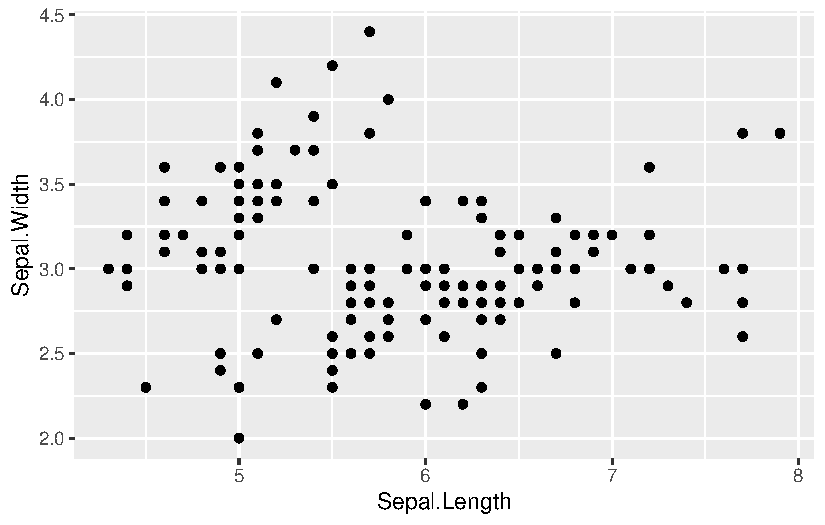
\includegraphics{AS_day5-tidyverse-template_files/figure-pdf/unnamed-chunk-6-1.pdf}

\subsection{Demo}\label{demo-2}

\subsubsection{The tidyverse philosophy}\label{the-tidyverse-philosophy}

\begin{Shaded}
\begin{Highlighting}[]
\NormalTok{iris }\SpecialCharTok{\%\textgreater{}\%}
    \FunctionTok{select}\NormalTok{(Sepal.Length, Sepal.Width, Species) }\SpecialCharTok{\%\textgreater{}\%}
    \FunctionTok{slice\_head}\NormalTok{(}\AttributeTok{n =} \DecValTok{3}\NormalTok{)}
\end{Highlighting}
\end{Shaded}

\begin{verbatim}
  Sepal.Length Sepal.Width Species
1          5.1         3.5  setosa
2          4.9         3.0  setosa
3          4.7         3.2  setosa
\end{verbatim}

\subsection{Exercise}\label{exercise}

\subsubsection{Read and write files}\label{read-and-write-files}

\begin{itemize}
\tightlist
\item
  Read data from the file \texttt{iris.csv}. Assign the data imported
  from the file to an object called \texttt{iris\_raw}.
\end{itemize}

\begin{Shaded}
\begin{Highlighting}[]
\FunctionTok{library}\NormalTok{(readr)}
\NormalTok{iris\_raw }\OtherTok{\textless{}{-}} \FunctionTok{read\_csv}\NormalTok{(}\StringTok{"/project/shared/r/1\_r\_data\_science/6{-}tidyverse/iris.csv"}\NormalTok{)}
\end{Highlighting}
\end{Shaded}

\begin{verbatim}
Rows: 150 Columns: 5
-- Column specification --------------------------------------------------------
Delimiter: ","
chr (1): species
dbl (4): sepal_length, sepal_width, petal_length, petal_width

i Use `spec()` to retrieve the full column specification for this data.
i Specify the column types or set `show_col_types = FALSE` to quiet this message.
\end{verbatim}

\textbf{What do you learn about the data from the messages displayed in
the R console while the contents of the file are parsed and imported
into your R session?}

\begin{quote}
Answer:
\end{quote}

\begin{itemize}
\tightlist
\item
  Print the value of \texttt{iris\_raw}.
\end{itemize}

\begin{Shaded}
\begin{Highlighting}[]
\FunctionTok{print}\NormalTok{(iris\_raw)}
\end{Highlighting}
\end{Shaded}

\begin{verbatim}
# A tibble: 150 x 5
   sepal_length sepal_width petal_length petal_width species    
          <dbl>       <dbl>        <dbl>       <dbl> <chr>      
 1          5.1         3.5          1.4         0.2 Iris-setosa
 2          4.9         3            1.4         0.2 Iris-setosa
 3          4.7         3.2          1.3         0.2 Iris-setosa
 4          4.6         3.1          1.5         0.2 Iris-setosa
 5          5           3.6          1.4         0.2 Iris-setosa
 6          5.4         3.9          1.7         0.4 Iris-setosa
 7          4.6         3.4          1.4         0.3 Iris-setosa
 8          5           3.4          1.5         0.2 Iris-setosa
 9          4.4         2.9          1.4         0.2 Iris-setosa
10          4.9         3.1          1.5         0.1 Iris-setosa
# i 140 more rows
\end{verbatim}

\begin{Shaded}
\begin{Highlighting}[]
\FunctionTok{str}\NormalTok{(iris\_raw)}
\end{Highlighting}
\end{Shaded}

\begin{verbatim}
spc_tbl_ [150 x 5] (S3: spec_tbl_df/tbl_df/tbl/data.frame)
 $ sepal_length: num [1:150] 5.1 4.9 4.7 4.6 5 5.4 4.6 5 4.4 4.9 ...
 $ sepal_width : num [1:150] 3.5 3 3.2 3.1 3.6 3.9 3.4 3.4 2.9 3.1 ...
 $ petal_length: num [1:150] 1.4 1.4 1.3 1.5 1.4 1.7 1.4 1.5 1.4 1.5 ...
 $ petal_width : num [1:150] 0.2 0.2 0.2 0.2 0.2 0.4 0.3 0.2 0.2 0.1 ...
 $ species     : chr [1:150] "Iris-setosa" "Iris-setosa" "Iris-setosa" "Iris-setosa" ...
 - attr(*, "spec")=
  .. cols(
  ..   sepal_length = col_double(),
  ..   sepal_width = col_double(),
  ..   petal_length = col_double(),
  ..   petal_width = col_double(),
  ..   species = col_character()
  .. )
 - attr(*, "problems")=<externalptr> 
\end{verbatim}

\begin{Shaded}
\begin{Highlighting}[]
\FunctionTok{dim}\NormalTok{(iris\_raw)}
\end{Highlighting}
\end{Shaded}

\begin{verbatim}
[1] 150   5
\end{verbatim}

\begin{Shaded}
\begin{Highlighting}[]
\FunctionTok{class}\NormalTok{(iris\_raw)}
\end{Highlighting}
\end{Shaded}

\begin{verbatim}
[1] "spec_tbl_df" "tbl_df"      "tbl"         "data.frame" 
\end{verbatim}

\begin{Shaded}
\begin{Highlighting}[]
\CommentTok{\# or just iris\_raw}
\end{Highlighting}
\end{Shaded}

\textbf{What is the class of the data? What are the dimensions of the
dataset? What is the type of data stored in each column?}

\begin{quote}
Answer:
\end{quote}

\begin{itemize}
\tightlist
\item
  Write the dataset to a file named \texttt{iris.tsv}, separating fields
  with the tabulation character.
\end{itemize}

\begin{Shaded}
\begin{Highlighting}[]
\FunctionTok{write\_tsv}\NormalTok{ (iris\_raw, }\StringTok{"iris.tsv"}\NormalTok{,}\AttributeTok{col\_names =} \ConstantTok{TRUE}\NormalTok{)}
\end{Highlighting}
\end{Shaded}

\textbf{What function do you use? What options are available for that
function?}

\begin{quote}
Answer:
\end{quote}

\begin{itemize}
\tightlist
\item
  Inspect the \texttt{iris.tsv} file. You can use \texttt{file.edit()}
  to open the file in the RStudio editor.
\end{itemize}

\begin{Shaded}
\begin{Highlighting}[]
\FunctionTok{file.edit}\NormalTok{( }\StringTok{"iris.tsv"}\NormalTok{ )}
\end{Highlighting}
\end{Shaded}

\textbf{Are you satisfied with the contents and appearance of the file?}

\begin{quote}
Answer:yes
\end{quote}

\subsection{Demo}\label{demo-3}

\subsubsection{Making a tibble}\label{making-a-tibble}

\begin{Shaded}
\begin{Highlighting}[]
\FunctionTok{tibble}\NormalTok{(}\AttributeTok{x =} \DecValTok{1}\SpecialCharTok{:}\DecValTok{5}\NormalTok{, }\AttributeTok{y =} \DecValTok{1}\NormalTok{, }\AttributeTok{z =}\NormalTok{ x }\SpecialCharTok{\^{}} \DecValTok{2} \SpecialCharTok{+}\NormalTok{ y)}
\end{Highlighting}
\end{Shaded}

\begin{verbatim}
# A tibble: 5 x 3
      x     y     z
  <int> <dbl> <dbl>
1     1     1     2
2     2     1     5
3     3     1    10
4     4     1    17
5     5     1    26
\end{verbatim}

\subsection{Demo}\label{demo-4}

\subsubsection{Subset the columns of a
table}\label{subset-the-columns-of-a-table}

\begin{Shaded}
\begin{Highlighting}[]
\NormalTok{iris }\SpecialCharTok{\%\textgreater{}\%}
    \FunctionTok{select}\NormalTok{(Sepal.Length, Sepal.Width) }\SpecialCharTok{\%\textgreater{}\%} 
    \FunctionTok{slice\_head}\NormalTok{(}\AttributeTok{n =} \DecValTok{6}\NormalTok{)}
\end{Highlighting}
\end{Shaded}

\begin{verbatim}
  Sepal.Length Sepal.Width
1          5.1         3.5
2          4.9         3.0
3          4.7         3.2
4          4.6         3.1
5          5.0         3.6
6          5.4         3.9
\end{verbatim}

\begin{Shaded}
\begin{Highlighting}[]
\CommentTok{\#slice head shows only the number in bracket}
\end{Highlighting}
\end{Shaded}

\begin{Shaded}
\begin{Highlighting}[]
\NormalTok{iris }\SpecialCharTok{\%\textgreater{}\%}
    \FunctionTok{select}\NormalTok{(}\FunctionTok{starts\_with}\NormalTok{(}\StringTok{"Petal"}\NormalTok{) }\SpecialCharTok{|} \FunctionTok{ends\_with}\NormalTok{(}\StringTok{"Width"}\NormalTok{)) }\SpecialCharTok{\%\textgreater{}\%} 
    \FunctionTok{slice\_head}\NormalTok{(}\AttributeTok{n =} \DecValTok{6}\NormalTok{)}
\end{Highlighting}
\end{Shaded}

\begin{verbatim}
  Petal.Length Petal.Width Sepal.Width
1          1.4         0.2         3.5
2          1.4         0.2         3.0
3          1.3         0.2         3.2
4          1.5         0.2         3.1
5          1.4         0.2         3.6
6          1.7         0.4         3.9
\end{verbatim}

\begin{Shaded}
\begin{Highlighting}[]
\CommentTok{\#shows all colums that start with petal and also those that end with width even if they did not start with petal}
\end{Highlighting}
\end{Shaded}

\begin{Shaded}
\begin{Highlighting}[]
\NormalTok{iris }\SpecialCharTok{\%\textgreater{}\%}
    \FunctionTok{select}\NormalTok{(}\SpecialCharTok{!}\FunctionTok{ends\_with}\NormalTok{(}\StringTok{"Width"}\NormalTok{)) }\SpecialCharTok{\%\textgreater{}\%} 
    \FunctionTok{slice\_head}\NormalTok{(}\AttributeTok{n =} \DecValTok{6}\NormalTok{)}
\end{Highlighting}
\end{Shaded}

\begin{verbatim}
  Sepal.Length Petal.Length Species
1          5.1          1.4  setosa
2          4.9          1.4  setosa
3          4.7          1.3  setosa
4          4.6          1.5  setosa
5          5.0          1.4  setosa
6          5.4          1.7  setosa
\end{verbatim}

\begin{Shaded}
\begin{Highlighting}[]
\CommentTok{\#removes all colums with width in its name}
\end{Highlighting}
\end{Shaded}

\begin{Shaded}
\begin{Highlighting}[]
\NormalTok{iris }\SpecialCharTok{\%\textgreater{}\%}
    \FunctionTok{select}\NormalTok{(}\SpecialCharTok{!}\FunctionTok{c}\NormalTok{(Sepal.Length, Petal.Length)) }\SpecialCharTok{\%\textgreater{}\%} 
    \FunctionTok{slice\_head}\NormalTok{(}\AttributeTok{n =} \DecValTok{6}\NormalTok{)}
\end{Highlighting}
\end{Shaded}

\begin{verbatim}
  Sepal.Width Petal.Width Species
1         3.5         0.2  setosa
2         3.0         0.2  setosa
3         3.2         0.2  setosa
4         3.1         0.2  setosa
5         3.6         0.2  setosa
6         3.9         0.4  setosa
\end{verbatim}

\begin{Shaded}
\begin{Highlighting}[]
\CommentTok{\#!c will not show those enlisted column but everything else}
\end{Highlighting}
\end{Shaded}

\subsection{Demo}\label{demo-5}

\subsubsection{Create and update columns in a
table}\label{create-and-update-columns-in-a-table}

\begin{Shaded}
\begin{Highlighting}[]
\NormalTok{iris }\SpecialCharTok{\%\textgreater{}\%}
    \FunctionTok{mutate}\NormalTok{(}
        \AttributeTok{ID =} \FunctionTok{seq}\NormalTok{(}\DecValTok{1}\NormalTok{, }\FunctionTok{nrow}\NormalTok{(iris)),}
        \AttributeTok{Flower.ID =} \FunctionTok{paste0}\NormalTok{(Species, ID)}
\NormalTok{        ) }\SpecialCharTok{\%\textgreater{}\%}
    \FunctionTok{slice\_head}\NormalTok{(}\AttributeTok{n =} \DecValTok{6}\NormalTok{)}
\end{Highlighting}
\end{Shaded}

\begin{verbatim}
  Sepal.Length Sepal.Width Petal.Length Petal.Width Species ID Flower.ID
1          5.1         3.5          1.4         0.2  setosa  1   setosa1
2          4.9         3.0          1.4         0.2  setosa  2   setosa2
3          4.7         3.2          1.3         0.2  setosa  3   setosa3
4          4.6         3.1          1.5         0.2  setosa  4   setosa4
5          5.0         3.6          1.4         0.2  setosa  5   setosa5
6          5.4         3.9          1.7         0.4  setosa  6   setosa6
\end{verbatim}

\begin{Shaded}
\begin{Highlighting}[]
\CommentTok{\#paste0 merges the info in the listed columns into 1 and displays it as new Flower.ID column, other \#column names ID created which sequentially numbers the row of hte specified database iris }
\end{Highlighting}
\end{Shaded}

\subsection{Demo}\label{demo-6}

\subsubsection{Subset observations in a
table}\label{subset-observations-in-a-table}

\begin{Shaded}
\begin{Highlighting}[]
\NormalTok{iris }\SpecialCharTok{\%\textgreater{}\%}
    \FunctionTok{filter}\NormalTok{(Sepal.Length }\SpecialCharTok{\textgreater{}} \FunctionTok{mean}\NormalTok{(Sepal.Length) }\SpecialCharTok{\&}\NormalTok{ Sepal.Width }\SpecialCharTok{\textgreater{}} \FunctionTok{mean}\NormalTok{(Sepal.Width)) }\SpecialCharTok{\%\textgreater{}\%}
    \FunctionTok{as\_tibble}\NormalTok{()}
\end{Highlighting}
\end{Shaded}

\begin{verbatim}
# A tibble: 25 x 5
   Sepal.Length Sepal.Width Petal.Length Petal.Width Species   
          <dbl>       <dbl>        <dbl>       <dbl> <fct>     
 1          7           3.2          4.7         1.4 versicolor
 2          6.4         3.2          4.5         1.5 versicolor
 3          6.9         3.1          4.9         1.5 versicolor
 4          6.3         3.3          4.7         1.6 versicolor
 5          6.7         3.1          4.4         1.4 versicolor
 6          5.9         3.2          4.8         1.8 versicolor
 7          6           3.4          4.5         1.6 versicolor
 8          6.7         3.1          4.7         1.5 versicolor
 9          6.3         3.3          6           2.5 virginica 
10          7.2         3.6          6.1         2.5 virginica 
# i 15 more rows
\end{verbatim}

\subsection{Demo}\label{demo-7}

\subsubsection{Compute summary
statistics}\label{compute-summary-statistics}

Without grouping

\begin{Shaded}
\begin{Highlighting}[]
\NormalTok{iris }\SpecialCharTok{\%\textgreater{}\%}
    \FunctionTok{summarise}\NormalTok{(}\AttributeTok{Sepal.Length.mean =} \FunctionTok{mean}\NormalTok{(Sepal.Length))}
\end{Highlighting}
\end{Shaded}

\begin{verbatim}
  Sepal.Length.mean
1          5.843333
\end{verbatim}

With grouping

\begin{Shaded}
\begin{Highlighting}[]
\NormalTok{iris }\SpecialCharTok{\%\textgreater{}\%}
    \FunctionTok{group\_by}\NormalTok{(Species) }\SpecialCharTok{\%\textgreater{}\%}
    \FunctionTok{summarise}\NormalTok{(}\AttributeTok{Sepal.Length.mean =} \FunctionTok{mean}\NormalTok{(Sepal.Length))}
\end{Highlighting}
\end{Shaded}

\begin{verbatim}
# A tibble: 3 x 2
  Species    Sepal.Length.mean
  <fct>                  <dbl>
1 setosa                  5.01
2 versicolor              5.94
3 virginica               6.59
\end{verbatim}

\subsection{Demo}\label{demo-8}

\subsubsection{Sort observations}\label{sort-observations}

\begin{Shaded}
\begin{Highlighting}[]
\NormalTok{iris }\SpecialCharTok{\%\textgreater{}\%}
    \FunctionTok{arrange}\NormalTok{(Species, }\FunctionTok{desc}\NormalTok{(Sepal.Length)) }\SpecialCharTok{\%\textgreater{}\%}
    \FunctionTok{as\_tibble}\NormalTok{()}
\end{Highlighting}
\end{Shaded}

\begin{verbatim}
# A tibble: 150 x 5
   Sepal.Length Sepal.Width Petal.Length Petal.Width Species
          <dbl>       <dbl>        <dbl>       <dbl> <fct>  
 1          5.8         4            1.2         0.2 setosa 
 2          5.7         4.4          1.5         0.4 setosa 
 3          5.7         3.8          1.7         0.3 setosa 
 4          5.5         4.2          1.4         0.2 setosa 
 5          5.5         3.5          1.3         0.2 setosa 
 6          5.4         3.9          1.7         0.4 setosa 
 7          5.4         3.7          1.5         0.2 setosa 
 8          5.4         3.9          1.3         0.4 setosa 
 9          5.4         3.4          1.7         0.2 setosa 
10          5.4         3.4          1.5         0.4 setosa 
# i 140 more rows
\end{verbatim}

\begin{Shaded}
\begin{Highlighting}[]
\CommentTok{\#sort observations}
\end{Highlighting}
\end{Shaded}

\subsection{Demo}\label{demo-9}

\subsubsection{Extract a single column as a
vector}\label{extract-a-single-column-as-a-vector}

Without names

\begin{Shaded}
\begin{Highlighting}[]
\NormalTok{iris }\SpecialCharTok{\%\textgreater{}\%}
    \FunctionTok{pull}\NormalTok{(Sepal.Length) }\SpecialCharTok{\%\textgreater{}\%}
    \FunctionTok{head}\NormalTok{(}\DecValTok{5}\NormalTok{)}
\end{Highlighting}
\end{Shaded}

\begin{verbatim}
[1] 5.1 4.9 4.7 4.6 5.0
\end{verbatim}

\begin{Shaded}
\begin{Highlighting}[]
\CommentTok{\# vector as in only values displayed}
\end{Highlighting}
\end{Shaded}

With names

\begin{Shaded}
\begin{Highlighting}[]
\NormalTok{iris }\SpecialCharTok{\%\textgreater{}\%}
    \FunctionTok{pull}\NormalTok{(Sepal.Length, }\AttributeTok{name =}\NormalTok{ Species) }\SpecialCharTok{\%\textgreater{}\%}
    \FunctionTok{head}\NormalTok{(}\DecValTok{5}\NormalTok{)}
\end{Highlighting}
\end{Shaded}

\begin{verbatim}
setosa setosa setosa setosa setosa 
   5.1    4.9    4.7    4.6    5.0 
\end{verbatim}

\begin{Shaded}
\begin{Highlighting}[]
\CommentTok{\#adds names to the pulled values, vector as in only values displayed}
\end{Highlighting}
\end{Shaded}

\subsection{Demo}\label{demo-10}

\subsubsection{Combine two tables using shared
information}\label{combine-two-tables-using-shared-information}

\begin{Shaded}
\begin{Highlighting}[]
\NormalTok{tibble\_1 }\OtherTok{\textless{}{-}} \FunctionTok{tibble}\NormalTok{(}
  \AttributeTok{ID =} \FunctionTok{paste0}\NormalTok{(}\StringTok{"sample"}\NormalTok{, }\DecValTok{1}\SpecialCharTok{:}\DecValTok{4}\NormalTok{),}
  \AttributeTok{gene1 =} \FunctionTok{rbinom}\NormalTok{(}\DecValTok{4}\NormalTok{, }\DecValTok{10}\NormalTok{, }\FloatTok{0.5}\NormalTok{),}
  \AttributeTok{gene2 =} \FunctionTok{rbinom}\NormalTok{(}\DecValTok{4}\NormalTok{, }\DecValTok{10}\NormalTok{, }\FloatTok{0.5}\NormalTok{)}
\NormalTok{)}
\NormalTok{tibble\_1}
\end{Highlighting}
\end{Shaded}

\begin{verbatim}
# A tibble: 4 x 3
  ID      gene1 gene2
  <chr>   <int> <int>
1 sample1     3     4
2 sample2     4     4
3 sample3     2     3
4 sample4     4     7
\end{verbatim}

\begin{Shaded}
\begin{Highlighting}[]
\NormalTok{tibble\_2 }\OtherTok{\textless{}{-}} \FunctionTok{tibble}\NormalTok{(}
  \AttributeTok{ID =} \FunctionTok{paste0}\NormalTok{(}\StringTok{"sample"}\NormalTok{, }\DecValTok{1}\SpecialCharTok{:}\DecValTok{4}\NormalTok{),}
  \AttributeTok{batch =} \FunctionTok{factor}\NormalTok{(}\FunctionTok{rep}\NormalTok{(}\FunctionTok{c}\NormalTok{(}\StringTok{"A"}\NormalTok{, }\StringTok{"B"}\NormalTok{), }\AttributeTok{each =} \DecValTok{2}\NormalTok{)),}
  \AttributeTok{condition =} \FunctionTok{factor}\NormalTok{(}\FunctionTok{rep}\NormalTok{(}\FunctionTok{c}\NormalTok{(}\StringTok{"control"}\NormalTok{, }\StringTok{"treated"}\NormalTok{), }\AttributeTok{times =} \DecValTok{2}\NormalTok{)),}
\NormalTok{)}
\NormalTok{tibble\_2}
\end{Highlighting}
\end{Shaded}

\begin{verbatim}
# A tibble: 4 x 3
  ID      batch condition
  <chr>   <fct> <fct>    
1 sample1 A     control  
2 sample2 A     treated  
3 sample3 B     control  
4 sample4 B     treated  
\end{verbatim}

\textbf{How would you describe how to join these two tibbles?}

\begin{Shaded}
\begin{Highlighting}[]
\NormalTok{tibble\_joined }\OtherTok{\textless{}{-}} \FunctionTok{left\_join}\NormalTok{(tibble\_1, tibble\_2, }\AttributeTok{by =} \StringTok{"ID"}\NormalTok{)}
\NormalTok{tibble\_joined}
\end{Highlighting}
\end{Shaded}

\begin{verbatim}
# A tibble: 4 x 5
  ID      gene1 gene2 batch condition
  <chr>   <int> <int> <fct> <fct>    
1 sample1     3     4 A     control  
2 sample2     4     4 A     treated  
3 sample3     2     3 B     control  
4 sample4     4     7 B     treated  
\end{verbatim}

\subsection{Exercise}\label{exercise-1}

\subsubsection{Manipulate data}\label{manipulate-data}

\paragraph{Exercise 1}\label{exercise-1-1}

\begin{itemize}
\tightlist
\item
  Using \texttt{iris\_raw}, for each species of iris, compute the
  following summary statistics for the \texttt{sepal\_length}: mean,
  median, minimum, maximum.
\end{itemize}

\begin{Shaded}
\begin{Highlighting}[]
\FunctionTok{library}\NormalTok{(dplyr)}
\NormalTok{iris\_raw }\SpecialCharTok{\%\textgreater{}\%} 
  \FunctionTok{group\_by}\NormalTok{(species) }\SpecialCharTok{\%\textgreater{}\%} 
  \FunctionTok{summarise}\NormalTok{(}\AttributeTok{mean\_sepal\_length =} \FunctionTok{mean}\NormalTok{(sepal\_length), }
            \AttributeTok{median\_sepal\_length =} \FunctionTok{median}\NormalTok{(sepal\_length),}
            \AttributeTok{minimum\_sepal\_length =} \FunctionTok{min}\NormalTok{(sepal\_length),}
            \AttributeTok{maximum\_sepal\_length =} \FunctionTok{max}\NormalTok{(sepal\_length)}
\NormalTok{            )}
\end{Highlighting}
\end{Shaded}

\begin{verbatim}
# A tibble: 3 x 5
  species         mean_sepal_length median_sepal_length minimum_sepal_length
  <chr>                       <dbl>               <dbl>                <dbl>
1 Iris-setosa                  5.01                 5                    4.3
2 Iris-versicolor              5.94                 5.9                  4.9
3 Iris-virginica               6.59                 6.5                  4.9
# i 1 more variable: maximum_sepal_length <dbl>
\end{verbatim}

\paragraph{Exercise 2}\label{exercise-2}

\begin{itemize}
\tightlist
\item
  For each species of iris, compute the mean of every column that is
  numeric. \textbf{Hint:} use the functions \texttt{dplyr::across()},
  \texttt{tidyselect::where()}, and \texttt{base::is.numeric()}.
\end{itemize}

\begin{Shaded}
\begin{Highlighting}[]
\CommentTok{\#base R way{-}{-}not what we want today}
\CommentTok{\#iris\_raw \%\textgreater{}\% select(!c(species)) \%\textgreater{}\% colMeans}
  
\CommentTok{\#iris\_raw \%\textgreater{}\% summarise(across(where(is.numeric))) \%\textgreater{}\% colmeans    {-}{-}wrong code}

\CommentTok{\#read help on across function ?across}
\NormalTok{iris\_raw }\SpecialCharTok{\%\textgreater{}\%} \FunctionTok{group\_by}\NormalTok{ (species) }\SpecialCharTok{\%\textgreater{}\%} \FunctionTok{summarise}\NormalTok{(}\FunctionTok{across}\NormalTok{(}\FunctionTok{where}\NormalTok{(is.numeric), mean))}
\end{Highlighting}
\end{Shaded}

\begin{verbatim}
# A tibble: 3 x 5
  species         sepal_length sepal_width petal_length petal_width
  <chr>                  <dbl>       <dbl>        <dbl>       <dbl>
1 Iris-setosa             5.01        3.42         1.46       0.244
2 Iris-versicolor         5.94        2.77         4.26       1.33 
3 Iris-virginica          6.59        2.97         5.55       2.03 
\end{verbatim}

\begin{itemize}
\tightlist
\item
  Filter the table above to retain only species of iris with an average
  sepal length less than \texttt{6}.
\end{itemize}

\begin{Shaded}
\begin{Highlighting}[]
\CommentTok{\# Copy the code chunk above and extend with more pipes}
\NormalTok{iris\_raw }\SpecialCharTok{\%\textgreater{}\%} 
  \FunctionTok{group\_by}\NormalTok{ (species) }\SpecialCharTok{\%\textgreater{}\%} 
  \FunctionTok{summarise}\NormalTok{(}\FunctionTok{across}\NormalTok{(}\FunctionTok{where}\NormalTok{(is.numeric), mean)) }\SpecialCharTok{\%\textgreater{}\%} 
  \FunctionTok{filter}\NormalTok{( sepal\_length }\SpecialCharTok{\textless{}} \DecValTok{6}\NormalTok{)}
\end{Highlighting}
\end{Shaded}

\begin{verbatim}
# A tibble: 2 x 5
  species         sepal_length sepal_width petal_length petal_width
  <chr>                  <dbl>       <dbl>        <dbl>       <dbl>
1 Iris-setosa             5.01        3.42         1.46       0.244
2 Iris-versicolor         5.94        2.77         4.26       1.33 
\end{verbatim}

\begin{Shaded}
\begin{Highlighting}[]
\CommentTok{\#you do not need to use the "by=" in the filter bracket because you already sorted it by species above.}
\CommentTok{\#you do not provide the data here in the filter bracket because you are piping input into it}
\end{Highlighting}
\end{Shaded}

\begin{itemize}
\tightlist
\item
  Sort the table above by descending \texttt{sepal\_length}.
\end{itemize}

\begin{Shaded}
\begin{Highlighting}[]
\CommentTok{\# Copy the code chunk above and extend with more pipes}
\NormalTok{iris\_raw }\SpecialCharTok{\%\textgreater{}\%} 
  \FunctionTok{group\_by}\NormalTok{ (species) }\SpecialCharTok{\%\textgreater{}\%} 
  \FunctionTok{summarise}\NormalTok{(}\FunctionTok{across}\NormalTok{(}\FunctionTok{where}\NormalTok{(is.numeric), mean)) }\SpecialCharTok{\%\textgreater{}\%} 
  \FunctionTok{filter}\NormalTok{( sepal\_length }\SpecialCharTok{\textless{}} \DecValTok{6}\NormalTok{) }\SpecialCharTok{\%\textgreater{}\%} 
  \FunctionTok{arrange}\NormalTok{(}\FunctionTok{desc}\NormalTok{(sepal\_length) )}
\end{Highlighting}
\end{Shaded}

\begin{verbatim}
# A tibble: 2 x 5
  species         sepal_length sepal_width petal_length petal_width
  <chr>                  <dbl>       <dbl>        <dbl>       <dbl>
1 Iris-versicolor         5.94        2.77         4.26       1.33 
2 Iris-setosa             5.01        3.42         1.46       0.244
\end{verbatim}

\begin{itemize}
\tightlist
\item
  From the table above, extract the \texttt{sepal\_length} column as a
  numeric vector. Make it a named numeric vector, where each value is
  named with the corresponding species.
\end{itemize}

\begin{Shaded}
\begin{Highlighting}[]
\CommentTok{\# Copy the code chunk above and extend with more pipes}
\NormalTok{iris\_raw }\SpecialCharTok{\%\textgreater{}\%} 
  \FunctionTok{group\_by}\NormalTok{ (species) }\SpecialCharTok{\%\textgreater{}\%} 
  \FunctionTok{summarise}\NormalTok{(}\FunctionTok{across}\NormalTok{(}\FunctionTok{where}\NormalTok{(is.numeric), mean)) }\SpecialCharTok{\%\textgreater{}\%} 
  \FunctionTok{filter}\NormalTok{( sepal\_length }\SpecialCharTok{\textless{}} \DecValTok{6}\NormalTok{) }\SpecialCharTok{\%\textgreater{}\%} 
  \FunctionTok{arrange}\NormalTok{(}\FunctionTok{desc}\NormalTok{(sepal\_length) ) }\SpecialCharTok{\%\textgreater{}\%} 
  \FunctionTok{pull}\NormalTok{ (sepal\_length, }\AttributeTok{name=}\NormalTok{species)}
\end{Highlighting}
\end{Shaded}

\begin{verbatim}
Iris-versicolor     Iris-setosa 
          5.936           5.006 
\end{verbatim}

\begin{Shaded}
\begin{Highlighting}[]
\CommentTok{\#name by species by name=species}
\end{Highlighting}
\end{Shaded}

\subsection{Exercise}\label{exercise-3}

\subsubsection{Manipulate data}\label{manipulate-data-1}

\paragraph{Exercise 3}\label{exercise-3-1}

Let's make the silly assumption that iris sepals are rectangular in
shape.

\begin{itemize}
\tightlist
\item
  Using \texttt{iris\_raw}, compute a new column named
  \texttt{sepal\_area}, which is the product of \texttt{sepal\_length}
  and \texttt{sepal\_width}.
\end{itemize}

\begin{Shaded}
\begin{Highlighting}[]
\NormalTok{iris\_raw }\SpecialCharTok{\%\textgreater{}\%} \FunctionTok{mutate}\NormalTok{(}\AttributeTok{sepal\_area=}\NormalTok{ sepal\_length}\SpecialCharTok{*}\NormalTok{sepal\_width )}
\end{Highlighting}
\end{Shaded}

\begin{verbatim}
# A tibble: 150 x 6
   sepal_length sepal_width petal_length petal_width species     sepal_area
          <dbl>       <dbl>        <dbl>       <dbl> <chr>            <dbl>
 1          5.1         3.5          1.4         0.2 Iris-setosa       17.8
 2          4.9         3            1.4         0.2 Iris-setosa       14.7
 3          4.7         3.2          1.3         0.2 Iris-setosa       15.0
 4          4.6         3.1          1.5         0.2 Iris-setosa       14.3
 5          5           3.6          1.4         0.2 Iris-setosa       18  
 6          5.4         3.9          1.7         0.4 Iris-setosa       21.1
 7          4.6         3.4          1.4         0.3 Iris-setosa       15.6
 8          5           3.4          1.5         0.2 Iris-setosa       17  
 9          4.4         2.9          1.4         0.2 Iris-setosa       12.8
10          4.9         3.1          1.5         0.1 Iris-setosa       15.2
# i 140 more rows
\end{verbatim}

\begin{itemize}
\tightlist
\item
  Subset the result to the columns named \texttt{species} and
  \texttt{sepal\_area}.
\end{itemize}

\begin{Shaded}
\begin{Highlighting}[]
\CommentTok{\# Copy the code chunk above and extend with more pipes}

\NormalTok{iris\_raw }\SpecialCharTok{\%\textgreater{}\%}
  \FunctionTok{mutate}\NormalTok{(}\AttributeTok{sepal\_area=}\NormalTok{ sepal\_length}\SpecialCharTok{*}\NormalTok{sepal\_width ) }\SpecialCharTok{\%\textgreater{}\%} 
  \FunctionTok{mutate}\NormalTok{(species, sepal\_area)}
\end{Highlighting}
\end{Shaded}

\begin{verbatim}
# A tibble: 150 x 6
   sepal_length sepal_width petal_length petal_width species     sepal_area
          <dbl>       <dbl>        <dbl>       <dbl> <chr>            <dbl>
 1          5.1         3.5          1.4         0.2 Iris-setosa       17.8
 2          4.9         3            1.4         0.2 Iris-setosa       14.7
 3          4.7         3.2          1.3         0.2 Iris-setosa       15.0
 4          4.6         3.1          1.5         0.2 Iris-setosa       14.3
 5          5           3.6          1.4         0.2 Iris-setosa       18  
 6          5.4         3.9          1.7         0.4 Iris-setosa       21.1
 7          4.6         3.4          1.4         0.3 Iris-setosa       15.6
 8          5           3.4          1.5         0.2 Iris-setosa       17  
 9          4.4         2.9          1.4         0.2 Iris-setosa       12.8
10          4.9         3.1          1.5         0.1 Iris-setosa       15.2
# i 140 more rows
\end{verbatim}

\begin{itemize}
\tightlist
\item
  Subset the result to display the top 5 observations by
  \texttt{sepal\_area}.
\end{itemize}

\begin{Shaded}
\begin{Highlighting}[]
\CommentTok{\# Copy the code chunk above and extend with more pipes}
\NormalTok{iris\_raw }\SpecialCharTok{\%\textgreater{}\%}
  \FunctionTok{mutate}\NormalTok{(}\AttributeTok{sepal\_area=}\NormalTok{ sepal\_length}\SpecialCharTok{*}\NormalTok{sepal\_width ) }\SpecialCharTok{\%\textgreater{}\%} 
  \FunctionTok{select}\NormalTok{(species, sepal\_area) }\SpecialCharTok{\%\textgreater{}\%} 
  \FunctionTok{slice\_max}\NormalTok{(sepal\_area, }\AttributeTok{n=}\DecValTok{5}\NormalTok{)}
\end{Highlighting}
\end{Shaded}

\begin{verbatim}
# A tibble: 5 x 2
  species        sepal_area
  <chr>               <dbl>
1 Iris-virginica       30.0
2 Iris-virginica       29.3
3 Iris-virginica       25.9
4 Iris-setosa          25.1
5 Iris-setosa          23.2
\end{verbatim}

\begin{Shaded}
\begin{Highlighting}[]
\CommentTok{\#slice\_head(n=5) does not sort it}
\CommentTok{\#slice\_max sorts it using order\_by}
\CommentTok{\#look at help page of all these function}
\end{Highlighting}
\end{Shaded}

\paragraph{Bonus point}\label{bonus-point}

\begin{itemize}
\tightlist
\item
  Make a histogram of \texttt{sepal\_area} colored by species.
\end{itemize}

You might also want to facet the plot by species.

\begin{Shaded}
\begin{Highlighting}[]
\CommentTok{\# Copy the code chunk above and extend with more pipes}
\FunctionTok{library}\NormalTok{(ggplot2)}

\NormalTok{iris\_for\_ggplot }\OtherTok{\textless{}{-}}\NormalTok{ iris\_raw }\SpecialCharTok{\%\textgreater{}\%}
  \FunctionTok{mutate}\NormalTok{(}\AttributeTok{sepal\_area=}\NormalTok{ sepal\_length}\SpecialCharTok{*}\NormalTok{sepal\_width ) }\SpecialCharTok{\%\textgreater{}\%} 
  \FunctionTok{select}\NormalTok{(species, sepal\_area) }\SpecialCharTok{\%\textgreater{}\%} 
  \FunctionTok{ggplot}\NormalTok{(}\FunctionTok{aes}\NormalTok{(}\AttributeTok{x=}\NormalTok{sepal\_area, }\AttributeTok{fill=}\NormalTok{species)) }\SpecialCharTok{+} 
  \FunctionTok{geom\_histogram}\NormalTok{ (}\AttributeTok{colour=}\StringTok{"black"}\NormalTok{)}\SpecialCharTok{+} 
  \FunctionTok{facet\_wrap}\NormalTok{(}\SpecialCharTok{\textasciitilde{}}\NormalTok{species, }\AttributeTok{nrow=}\DecValTok{2}\NormalTok{) }\SpecialCharTok{+}
  \FunctionTok{labs}\NormalTok{(}\AttributeTok{title=}\StringTok{"Sepal area\_Iris dataset"}\NormalTok{, }\AttributeTok{x=} \StringTok{"Sepal area"}\NormalTok{, }\AttributeTok{y=}\StringTok{"Observation"}\NormalTok{) }\SpecialCharTok{+} \FunctionTok{theme}\NormalTok{(}\AttributeTok{axis.text=}\FunctionTok{element\_text}\NormalTok{(}\AttributeTok{size=}\DecValTok{9}\NormalTok{),}\AttributeTok{axis.line =} \FunctionTok{element\_line}\NormalTok{(}\AttributeTok{size=}\FloatTok{0.5}\NormalTok{), }\AttributeTok{axis.title =} \FunctionTok{element\_text}\NormalTok{(}\AttributeTok{size=}\DecValTok{12}\NormalTok{), }\AttributeTok{plot.title=}\FunctionTok{element\_text}\NormalTok{(}\AttributeTok{hjust=}\FloatTok{0.5}\NormalTok{))}
\end{Highlighting}
\end{Shaded}

\begin{verbatim}
Warning: The `size` argument of `element_line()` is deprecated as of ggplot2 3.4.0.
i Please use the `linewidth` argument instead.
\end{verbatim}

\begin{Shaded}
\begin{Highlighting}[]
\NormalTok{iris\_for\_ggplot}
\end{Highlighting}
\end{Shaded}

\begin{verbatim}
`stat_bin()` using `bins = 30`. Pick better value with `binwidth`.
\end{verbatim}

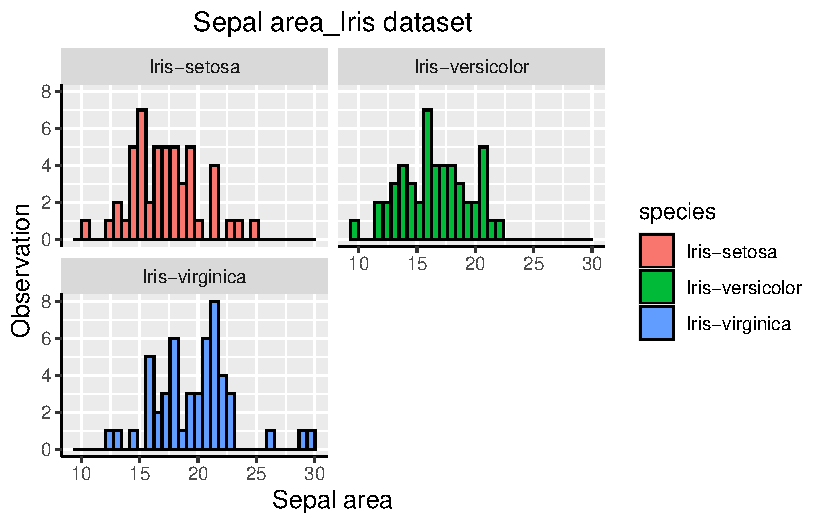
\includegraphics{AS_day5-tidyverse-template_files/figure-pdf/unnamed-chunk-35-1.pdf}

\begin{Shaded}
\begin{Highlighting}[]
\CommentTok{\#ggplot(iris\_for\_ggplot,  )}

\CommentTok{\#i dont know what to do}
\end{Highlighting}
\end{Shaded}

\subsection{Exercise}\label{exercise-4}

\subsubsection{Pivot data from wide to
long}\label{pivot-data-from-wide-to-long}

Reshape the \texttt{iris\_raw} dataset in a tidy format where one
observation is represented by:

\begin{itemize}
\item
  the species
\item
  the variable measured
\item
  the value
\end{itemize}

\textbf{Hint:} you want to pivot all the columns that start are numeric.

\begin{Shaded}
\begin{Highlighting}[]
\CommentTok{\#iris\_long \textless{}{-} iris\_raw \%\textgreater{}\% pivot\_longer(across(where(cols(species, is.numeric)))}
\CommentTok{\#iris\_long \textless{}{-} iris\_raw \%\textgreater{}\% pivot\_longer(cols(where(species, is.numeric)))}
\CommentTok{\#iris\_long \textless{}{-} iris\_raw \%\textgreater{}\% pivot\_longer(cols(is.numeric))}
\CommentTok{\#iris\_long \textless{}{-} iris\_raw \%\textgreater{}\% pivot\_longer(cols = starts\_with ("sepal", "petal", "species"))}
\CommentTok{\#iris\_long \textless{}{-} iris\_raw \%\textgreater{}\% pivot\_longer(starts\_with ("sepal", "petal", "species"))}
\NormalTok{iris\_long }\OtherTok{\textless{}{-}}\NormalTok{ iris\_raw }\SpecialCharTok{\%\textgreater{}\%} \FunctionTok{pivot\_longer}\NormalTok{(}\FunctionTok{where}\NormalTok{(is.numeric))}
\NormalTok{iris\_long}
\end{Highlighting}
\end{Shaded}

\begin{verbatim}
# A tibble: 600 x 3
   species     name         value
   <chr>       <chr>        <dbl>
 1 Iris-setosa sepal_length   5.1
 2 Iris-setosa sepal_width    3.5
 3 Iris-setosa petal_length   1.4
 4 Iris-setosa petal_width    0.2
 5 Iris-setosa sepal_length   4.9
 6 Iris-setosa sepal_width    3  
 7 Iris-setosa petal_length   1.4
 8 Iris-setosa petal_width    0.2
 9 Iris-setosa sepal_length   4.7
10 Iris-setosa sepal_width    3.2
# i 590 more rows
\end{verbatim}

\begin{Shaded}
\begin{Highlighting}[]
\CommentTok{\#iris\_raw}
\end{Highlighting}
\end{Shaded}

\textbf{What information have we lost in the process? What could we do
to remedy the issue?}

\begin{quote}
Answer: The identity of each observation is lost; e.g., we cannot tell
which value of \texttt{sepal\_length} is associated with which value of
\texttt{sepal\_width}.
\end{quote}

\begin{Shaded}
\begin{Highlighting}[]
\CommentTok{\# Copy the code chunk above and refine to address the issue}
\NormalTok{iris\_long2  }\OtherTok{\textless{}{-}}\NormalTok{ iris\_raw  }\SpecialCharTok{\%\textgreater{}\%} 
  \FunctionTok{mutate}\NormalTok{(}\AttributeTok{id =} \FunctionTok{as.character}\NormalTok{(}\FunctionTok{row\_number}\NormalTok{())) }\SpecialCharTok{\%\textgreater{}\%} 
  \FunctionTok{pivot\_longer}\NormalTok{(}\FunctionTok{where}\NormalTok{(is.numeric))}
\NormalTok{iris\_long2}
\end{Highlighting}
\end{Shaded}

\begin{verbatim}
# A tibble: 600 x 4
   species     id    name         value
   <chr>       <chr> <chr>        <dbl>
 1 Iris-setosa 1     sepal_length   5.1
 2 Iris-setosa 1     sepal_width    3.5
 3 Iris-setosa 1     petal_length   1.4
 4 Iris-setosa 1     petal_width    0.2
 5 Iris-setosa 2     sepal_length   4.9
 6 Iris-setosa 2     sepal_width    3  
 7 Iris-setosa 2     petal_length   1.4
 8 Iris-setosa 2     petal_width    0.2
 9 Iris-setosa 3     sepal_length   4.7
10 Iris-setosa 3     sepal_width    3.2
# i 590 more rows
\end{verbatim}

\begin{Shaded}
\begin{Highlighting}[]
\CommentTok{\#names\_to="variable" in pivot longer assign}
\CommentTok{\#mutate(rowid\_to\_column(var=rowid))not this}
\CommentTok{\#mutate(specimen = (row\_number()){-}{-}{-}kevin did this}
\end{Highlighting}
\end{Shaded}

\subsection{Exercise}\label{exercise-5}

\subsubsection{Pivot data from long to
wide}\label{pivot-data-from-long-to-wide}

\begin{itemize}
\tightlist
\item
  Reshape the tidy format of the iris data set into the original wide
  format.
\end{itemize}

\textbf{Hint:} you will only be able to restore the wide format if you
kept track of the identity of each flower in the long format.

\begin{Shaded}
\begin{Highlighting}[]
\NormalTok{iris\_long2 }\SpecialCharTok{\%\textgreater{}\%} 
 \FunctionTok{pivot\_wider}\NormalTok{(}\AttributeTok{names\_from =}\NormalTok{ name, }\AttributeTok{values\_from =}\NormalTok{ value, )}
\end{Highlighting}
\end{Shaded}

\begin{verbatim}
# A tibble: 150 x 6
   species     id    sepal_length sepal_width petal_length petal_width
   <chr>       <chr>        <dbl>       <dbl>        <dbl>       <dbl>
 1 Iris-setosa 1              5.1         3.5          1.4         0.2
 2 Iris-setosa 2              4.9         3            1.4         0.2
 3 Iris-setosa 3              4.7         3.2          1.3         0.2
 4 Iris-setosa 4              4.6         3.1          1.5         0.2
 5 Iris-setosa 5              5           3.6          1.4         0.2
 6 Iris-setosa 6              5.4         3.9          1.7         0.4
 7 Iris-setosa 7              4.6         3.4          1.4         0.3
 8 Iris-setosa 8              5           3.4          1.5         0.2
 9 Iris-setosa 9              4.4         2.9          1.4         0.2
10 Iris-setosa 10             4.9         3.1          1.5         0.1
# i 140 more rows
\end{verbatim}

\subsection{Demo}\label{demo-11}

\subsubsection{Split a column value into multiple
columns}\label{split-a-column-value-into-multiple-columns}

\begin{Shaded}
\begin{Highlighting}[]
\NormalTok{iris }\SpecialCharTok{\%\textgreater{}\%} 
    \FunctionTok{separate}\NormalTok{(Sepal.Length, }\FunctionTok{c}\NormalTok{(}\StringTok{"Sepal.Length.unit"}\NormalTok{, }\StringTok{"Sepal.Length.decimal"}\NormalTok{), }\AttributeTok{sep =} \StringTok{"[.]"}\NormalTok{) }\SpecialCharTok{\%\textgreater{}\%}
    \FunctionTok{select}\NormalTok{(}\FunctionTok{c}\NormalTok{(}\StringTok{"Sepal.Length.unit"}\NormalTok{, }\StringTok{"Sepal.Length.decimal"}\NormalTok{)) }\SpecialCharTok{\%\textgreater{}\%}
    \FunctionTok{as\_tibble}\NormalTok{()}
\end{Highlighting}
\end{Shaded}

\begin{verbatim}
Warning: Expected 2 pieces. Missing pieces filled with `NA` in 17 rows [5, 8, 26, 27,
36, 41, 44, 50, 51, 61, 63, 79, 84, 86, 94, 120, 139].
\end{verbatim}

\begin{verbatim}
# A tibble: 150 x 2
   Sepal.Length.unit Sepal.Length.decimal
   <chr>             <chr>               
 1 5                 1                   
 2 4                 9                   
 3 4                 7                   
 4 4                 6                   
 5 5                 <NA>                
 6 5                 4                   
 7 4                 6                   
 8 5                 <NA>                
 9 4                 4                   
10 4                 9                   
# i 140 more rows
\end{verbatim}

\subsection{Demo}\label{demo-12}

\subsubsection{Combine multiple columns into a single
value}\label{combine-multiple-columns-into-a-single-value}

\begin{Shaded}
\begin{Highlighting}[]
\NormalTok{iris }\SpecialCharTok{\%\textgreater{}\%} 
  \FunctionTok{mutate}\NormalTok{(}\AttributeTok{ID =} \FunctionTok{seq}\NormalTok{(}\DecValTok{1}\NormalTok{, }\FunctionTok{nrow}\NormalTok{(iris))) }\SpecialCharTok{\%\textgreater{}\%} 
  \FunctionTok{unite}\NormalTok{(}\StringTok{"FlowerID"}\NormalTok{, Species, ID, }\AttributeTok{sep =} \StringTok{"\_"}\NormalTok{) }\SpecialCharTok{\%\textgreater{}\%} 
  \FunctionTok{as\_tibble}\NormalTok{()}
\end{Highlighting}
\end{Shaded}

\begin{verbatim}
# A tibble: 150 x 5
   Sepal.Length Sepal.Width Petal.Length Petal.Width FlowerID 
          <dbl>       <dbl>        <dbl>       <dbl> <chr>    
 1          5.1         3.5          1.4         0.2 setosa_1 
 2          4.9         3            1.4         0.2 setosa_2 
 3          4.7         3.2          1.3         0.2 setosa_3 
 4          4.6         3.1          1.5         0.2 setosa_4 
 5          5           3.6          1.4         0.2 setosa_5 
 6          5.4         3.9          1.7         0.4 setosa_6 
 7          4.6         3.4          1.4         0.3 setosa_7 
 8          5           3.4          1.5         0.2 setosa_8 
 9          4.4         2.9          1.4         0.2 setosa_9 
10          4.9         3.1          1.5         0.1 setosa_10
# i 140 more rows
\end{verbatim}

\subsection{Demo}\label{demo-13}

\subsubsection{Extract substrings}\label{extract-substrings}

\begin{Shaded}
\begin{Highlighting}[]
\NormalTok{iris\_species }\OtherTok{\textless{}{-}}\NormalTok{ iris }\SpecialCharTok{\%\textgreater{}\%}
    \FunctionTok{pull}\NormalTok{(Species)}
\end{Highlighting}
\end{Shaded}

\begin{Shaded}
\begin{Highlighting}[]
\NormalTok{iris\_species }\SpecialCharTok{\%\textgreater{}\%}
    \FunctionTok{str\_sub}\NormalTok{(}\DecValTok{1}\NormalTok{, }\DecValTok{3}\NormalTok{) }\SpecialCharTok{\%\textgreater{}\%}
    \FunctionTok{unique}\NormalTok{()}
\end{Highlighting}
\end{Shaded}

\begin{verbatim}
[1] "set" "ver" "vir"
\end{verbatim}

\begin{Shaded}
\begin{Highlighting}[]
\CommentTok{\#answer "set" "ver" "vir"}
\end{Highlighting}
\end{Shaded}

\begin{Shaded}
\begin{Highlighting}[]
\FunctionTok{str\_sub}\NormalTok{(iris\_species, }\DecValTok{4}\NormalTok{) }\OtherTok{\textless{}{-}} \StringTok{"..."}
\NormalTok{iris\_species }\SpecialCharTok{\%\textgreater{}\%}
    \FunctionTok{unique}\NormalTok{()}
\end{Highlighting}
\end{Shaded}

\begin{verbatim}
[1] "set..." "ver..." "vir..."
\end{verbatim}

\begin{Shaded}
\begin{Highlighting}[]
\CommentTok{\#answer"set..." "ver..." "vir..."}
\end{Highlighting}
\end{Shaded}

\subsection{Demo}\label{demo-14}

\subsubsection{Join multiple strings and remove
whitespaces}\label{join-multiple-strings-and-remove-whitespaces}

\begin{Shaded}
\begin{Highlighting}[]
\NormalTok{words }\OtherTok{\textless{}{-}} \FunctionTok{c}\NormalTok{(}\StringTok{"A "}\NormalTok{, }\StringTok{" few "}\NormalTok{, }\StringTok{"words"}\NormalTok{)}
\NormalTok{words}
\end{Highlighting}
\end{Shaded}

\begin{verbatim}
[1] "A "    " few " "words"
\end{verbatim}

\begin{Shaded}
\begin{Highlighting}[]
\NormalTok{words }\SpecialCharTok{\%\textgreater{}\%}
    \FunctionTok{str\_trim}\NormalTok{()}
\end{Highlighting}
\end{Shaded}

\begin{verbatim}
[1] "A"     "few"   "words"
\end{verbatim}

\begin{Shaded}
\begin{Highlighting}[]
\CommentTok{\#"A"     "few"   "words" removed the spaces within the quotes}
\end{Highlighting}
\end{Shaded}

\begin{Shaded}
\begin{Highlighting}[]
\NormalTok{words }\SpecialCharTok{\%\textgreater{}\%}
    \FunctionTok{str\_trim}\NormalTok{() }\SpecialCharTok{\%\textgreater{}\%}
    \FunctionTok{str\_c}\NormalTok{(}\AttributeTok{collapse =} \StringTok{" "}\NormalTok{)}
\end{Highlighting}
\end{Shaded}

\begin{verbatim}
[1] "A few words"
\end{verbatim}

\begin{Shaded}
\begin{Highlighting}[]
\CommentTok{\#collapses brings them together}
\end{Highlighting}
\end{Shaded}





\end{document}
